\documentclass{article}
\usepackage[utf8]{inputenc}
\usepackage{amstext}
\usepackage{amsmath} 
\usepackage{mathpazo}
\usepackage{graphicx} 
\usepackage{float} 
\usepackage{caption} 
\usepackage{epstopdf} 
\usepackage{hyperref}
\usepackage{varioref} 
\usepackage{fancyref}
\usepackage[section]{placeins} 
\usepackage{perpage}
\usepackage[margin=1in, paperwidth=8.5in, paperheight=11in]{geometry} 
\MakeSorted{figure} 
\usepackage{natbib}
\usepackage{graphicx}
\usepackage{xcolor}
\usepackage{listings}
\usepackage{minted}
\usepackage{subcaption}
\usepackage{eso-pic}
\usepackage{tikz}
\usepackage[american]{circuitikz}
\usepackage[font=small,labelfont=bf]{caption}

\title{ENGR2420 Lab 7 : The MOS Differential Pair}
\author{Abigail Fry\\ Anusha Datar\\ Vienna Scheyer}
\date{April 15, 2019}

\begin{document}

\maketitle

\section{Experiment One : Differential Pair Current–Voltage Characteristics}
In this experiment, we measured the current-voltage characteristics of an nMOS differential pair at varying values of the common-mode input voltage and as a function of bias current levels while varying gate voltages for one of the transistors in the pair.  We constructed our differential pair out of transistors on the ALD1106 nMOS array. 

\begin{figure}[H]
  \begin{center}      
  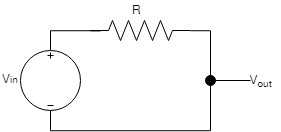
\includegraphics[scale = 0.5]{images/exp1_schematic.jpg}
  \caption{Schematic for the circuit used to characterize the nMOS differential pair.}   
  \label{fig:exp1_schematic}
  \end{center}
\end{figure}

\subsection{Results}
We first plotted the values $I_1$, $I_2$, $I_1$+$I_2$, and $I_1$-$I_2$ as a function of $V_1$-$V_2$, or $V_{dm}$, for each value of $V_2$ when $V_b$ was at the threshold voltage, 0.65 V.
\begin{figure}[H]
  \begin{center}       
  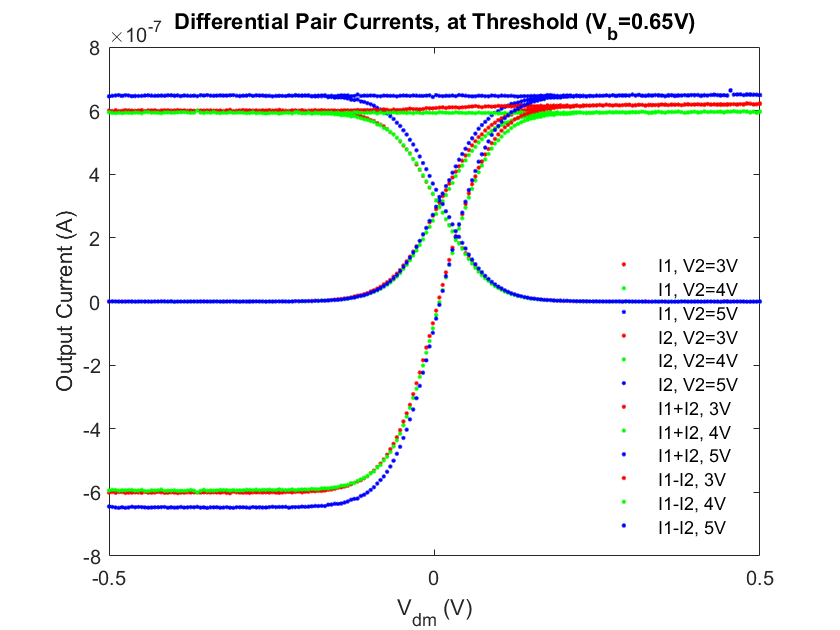
\includegraphics[scale = 0.5]{images/current_thresh.png}
  \caption{Output current as a function of $V_{dm}$ for nMOS differential pair.}   
  \label{fig:exp1_below_current}
  \end{center}
\end{figure}
Then, we plotted the voltage at the common source node for each value of $V_2$. 
\begin{figure}[H]
  \begin{center}       
  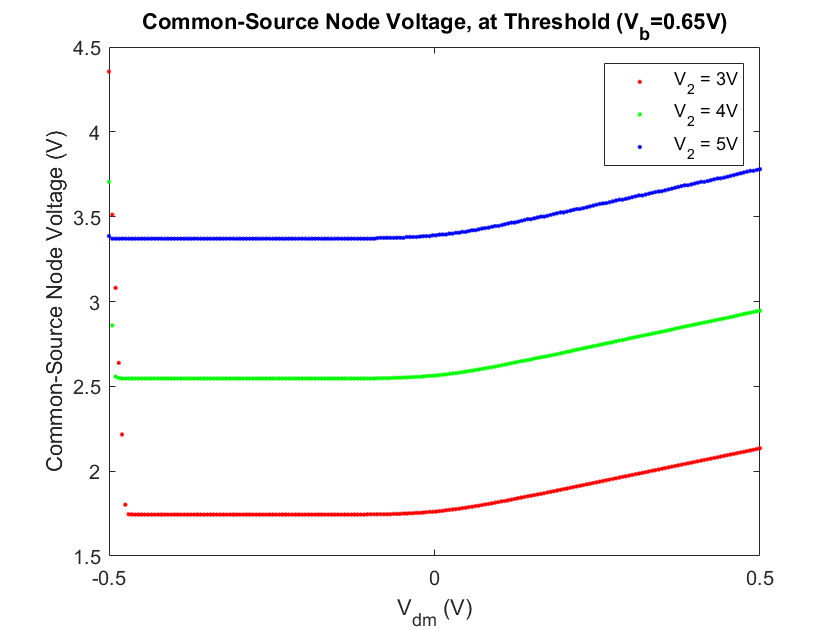
\includegraphics[scale = 0.5]{images/threshold_cm_node.png}
  \caption{Common-source node voltage as a function of $V_{dm}$ for nMOS differential pair.}   
  \label{fig:exp1_below_voltage}
  \end{center}
\end{figure}
We also plotted the incremental differential mode transconductance gain of the differential pair at threshold, as shown in Figure \ref{fig: Gdm}.
\begin{figure}[H]
  \begin{center}       
  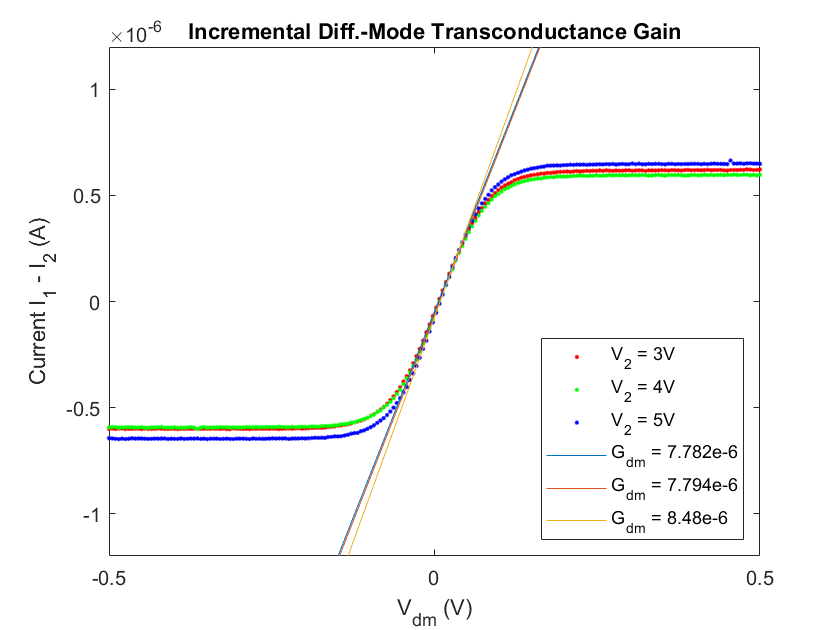
\includegraphics[scale = 0.5]{images/Gdm.png}
  \caption{$G_{dm}$ extracted from current-voltage characteristics of nMOS differential pair at threshold.}   
  \label{fig:exp1_below_voltage}
  \label{fig: Gdm}
  \end{center}
\end{figure}

Next, we set the bias voltage to 1.5 Volts so that the bias current was above the threshold. Then, we set the value of $ V_{2}$ to 5V. We measured the currents and the common source node voltages for the differential pair. To see the full range of behavior, we swept a range from -1 V to 1 V for voltage at $V_{dm}$. We plotted output current as a function of $V_{dm}$ for the differential pair above threshold, as seen in Figure \ref{fig:above_v}.

\begin{figure}[H]
  \begin{center}       
  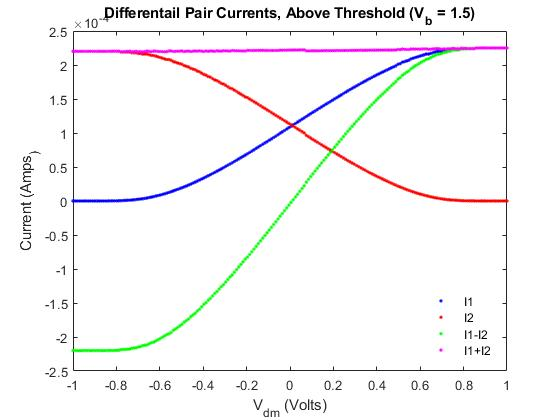
\includegraphics[scale = 0.5]{images/above_c_u.jpg}
  \caption{Currents as a function of $ V_{dm}$ when bias current is above threshold}   
  \label{fig:above_v}
  \end{center}
\end{figure}

We plotted common-source node voltage as a function of $V_{dm}$ on linear axes as seen in Figure \ref{fig:above_c}.

\begin{figure}[H]
  \begin{center}       
  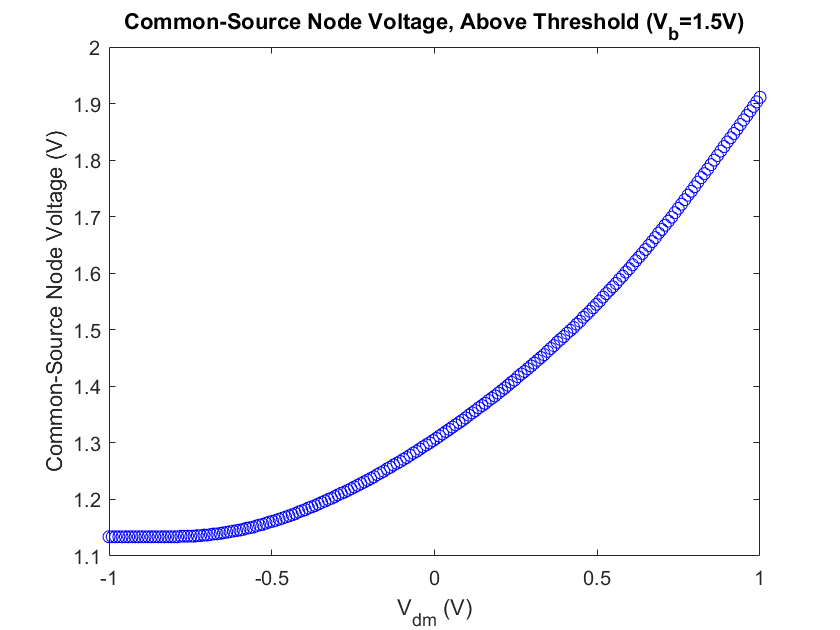
\includegraphics[scale = 0.5]{images/above_thresh_cm_node.png}
  \caption{Common-source node voltage as a function $V_{dm}$ when bias current is above threshold.}   
  \label{fig:above_c}
  \end{center}
\end{figure}

\subsection{Analysis}
%% Below threshold analysis
To start, we studied the differential pair with $V_b = 0.65V$, or at the threshold voltage. Theoretically, a lower $V_2$ should lead to slightly lower current values for both $I_1$ and $I_2$, but the behavior should remain consistent regardless of the value of $V_2$ - the current should quickly increase from negative to positive around $V_{dm} = 0$ V. Meanwhile, the value of the common source node voltage should increase proportionally as $V_2$ increases but the behavior should be consistent, with constant voltage when $V_2 < V_1$ and a linear relationship when  $V_2 > V_1$. Our experimental results qualitatively reflect this behavior. 
%% Transconductance analysis
\newline
The definition of incremental differential-mode transconductance gain is formally given as follows: 
\begin{center}
 $G_{dm} = \frac{\delta I_{dm}}{\delta V_{dm}} | \bigg\revert_{V_{dm}=0} = \frac{\delta (I_1 - I_2)}{\delta (V_1 - V_2)} | \bigg\revert_{V_{dm}=0}$
\end{center}

We fit a line to the linear region of the $I_1-I_2$ plot, which is the section of the data near the point where $V_1 - V_2 = 0$. By taking the slope of this line, we extracted the incremental differential-mode transconductance gain at each value of $V_2$, as shown in Figure \ref{fig: Gdm}.
%% Above threshold analysis
\newline
Theoretically, in the current-voltage characteristic plot for above threshold, $I_{1}$ and  $I_{2}$ should be mirrors of one another and intersect at 0 V.  We expected that the $I_{1}$ - $I_{2}$ would pass through the point (0,0) on the plot.  For the voltage plots, the threshold plot would not follow the soft max function and instead follow an exponential trend.

\subsection{Discussion}
%% Below threshold discussion
The current-voltage characteristics change somewhat as $V_2$ changes, and the most noticeable difference is that when $V_2=5V$ the current diverges slightly more, but is still very close in value. Overall, the starting values and slopes are very similar.  The current for $I_{1}$ and $I_{2}$ also rail high to about $6e-7$ amps and rail low to 0 amps.
 In the case of the common source node voltage, when $V_1$ goes from below $V_2$ to above it, the value of $V_{dm}$ as a function of common source node voltage goes from flat lining to having a slope of $0.78$, $0.79$, and $0.81$ for each value of $V_2$, respectively. Note that these slope values are dimensionless because these are ratios of $volts$ over $volts$. In other words, $V_{dm}$ does not change when $V_1$ is less than $V_2$, but $V_{dm}$ as a function of common source node voltage has a positive slope when $V_1$ exceeds $V_2$.
 
The value of the differential-mode transconductance gain changes from 7.82e-6 for $V_2=3V$ to 7.94e-6 for $V_2=4V$ to 8.48e-6 for $V_2=5V$. Again, the differential-mode transconductance gain when $V_2$ is $3V$ and $4$V is close together, and when $V_2$ is $5V$ the value is noticeably larger.
%% Above threshold discussion

The current-voltage characteristic plot of the circuit below threshold, Figure \ref{fig:exp1_below_current}, and the plot above threshold, Figure \ref{fig:above_c}, are similar in many ways.  $I_{1}$ and $I_{2}$ are mirror images of one another and intersect at 0 volts.  To be able to see the full current behavior at above threshold, we did have to sweep a wider range for $V_{dm}$ than when the circuit was below threshold.  Without the larger range, some of the current behavior would have been cut off. For the below threshold plots, the currents of $I_{1}$ and $I_{2}$ rail for a longer range of voltages.  At above threshold, the transition region is longer because the bias current is higher at strong inversion and it takes longer to saturate.

The distinction between each of the common-source node voltages as a function of $V_{dm}$ for each value of $V_b$ is that the below threshold current plot follows the soft max function and the above threshold plot follows more of an exponential function.
\
\end{document}
